\documentclass{beamer}

\usepackage{comment}
\usepackage{color}
\usepackage{listings}
\usepackage{verbatim}
\usepackage{multicol}
\usepackage{booktabs}
\definecolor{green}{RGB}{0,128,0}

\def\EQ#1\EN{\begin{equation*}#1\end{equation*}}
\def\BA#1\EA{\begin{align*}#1\end{align*}}
\def\BS#1\ES{\begin{split*}#1\end{split*}}
\newcommand{\bc}{\begin{center}}
\newcommand{\ec}{\end{center}}
\newcommand{\eq}{\ =\ }
\newcommand{\degc}{$^\circ$C}

\def\p{\partial}
\def\qbs{\boldsymbol{q}}
\def\Dbs{\boldsymbol{D}}
\def\A{\mathcal A}
\def\gC{\mathcal C}
\def\gD{\mathcal D}
\def\gL{\mathcal L}
\def\M{\mathcal M}
\def\P{\mathcal P}
\def\Q{\mathcal Q}
\def\gR{\mathcal R}
\def\gS{\mathcal S}
\def\X{\mathcal X}
\def\bnabla{\boldsymbol{\nabla}}
\def\bnu{\boldsymbol{\nu}}
\renewcommand{\a}{{\alpha}}
%\renewcommand{\a}{{}}
\newcommand{\s}{{\sigma}}
\newcommand{\bq}{\boldsymbol{q}}
\newcommand{\bz}{\boldsymbol{z}}
\def\bPsi{\boldsymbol{\Psi}}

\def\Li{\textit{L}}
\def\Fb{\textbf{f}}
\def\Jb{\textbf{J}}
\def\cb{\textbf{c}}

\def\Dt{\Delta t}
\def\tpdt{{t + \Delta t}}
\def\bpsi{\boldsymbol{\psi}}
\def\dbpsi{\delta \boldsymbol{\psi}}
\def\bc{\textbf{c}}
\def\dbc{\delta \textbf{c}}
\def\arrows{\rightleftharpoons}

\newcommand{\bGamma}{\boldsymbol{\Gamma}}
\newcommand{\bOmega}{\boldsymbol{\Omega}}
%\newcommand{\bPsi}{\boldsymbol{\Psi}}
%\newcommand{\bpsi}{\boldsymbol{\psi}}
\newcommand{\bO}{\boldsymbol{O}}
%\newcommand{\bnu}{\boldsymbol{\nu}}
\newcommand{\bdS}{\boldsymbol{dS}}
\newcommand{\bg}{\boldsymbol{g}}
\newcommand{\bk}{\boldsymbol{k}}
%\newcommand{\bq}{\boldsymbol{q}}
\newcommand{\br}{\boldsymbol{r}}
\newcommand{\bR}{\boldsymbol{R}}
\newcommand{\bS}{\boldsymbol{S}}
\newcommand{\bu}{\boldsymbol{u}}
\newcommand{\bv}{\boldsymbol{v}}
%\newcommand{\bz}{\boldsymbol{z}}
\newcommand{\pressure}{P}

\def\water{H$_2$O}
\def\calcium{Ca$^{2+}$}
\def\copper{Cu$^{2+}$}
\def\magnesium{Mg$^{2+}$}
\def\sodium{Na$^+$}
\def\potassium{K$^+$}
\def\uranium{UO$_2^{2+}$}
\def\hion{H$^+$}
\def\hydroxide{0H$^-$}
\def\bicarbonate{HCO$_3^-$}
\def\carbonate{CO$_3^{2-}$}
\def\cotwo{CO$_2$(aq)}
\def\chloride{Cl$^-$}
\def\fluoride{F$^-$}
\def\phosphoricacid{HPO$_4^{2-}$}
\def\nitrate{NO$_3^-$}
\def\sulfate{SO$_4^{2-}$}
\def\souotwooh{$>$SOUO$_2$OH}
\def\sohuotwocothree{$>$SOHUO$_2$CO$_3$}
\def\soh{$>$SOH}

\newcommand\gehcomment[1]{{{\color{orange} #1}}}
\newcommand\add[1]{{{\color{blue} #1}}}
\newcommand\remove[1]{\sout{{\color{red} #1}}}
\newcommand\codecomment[1]{{{\color{green} #1}}}
\newcommand\redcomment[1]{{{\color{red} #1}}}
\newcommand\bluecomment[1]{{{\color{blue} #1}}}
\newcommand\greencomment[1]{{{\color{green} #1}}}
\newcommand\magentacomment[1]{{{\color{magenta} #1}}}

\begin{comment}
\tiny
\scriptsize
\footnotesize
\small
\normalsize
\large
\Large
\LARGE
\huge
\Huge
\end{comment}

\begin{document}
\title{2D Density Dependent Flow Scenario in a Nutshell}
\author{Glenn Hammond}
\date{\today}

%\frame{\titlepage}

%-----------------------------------------------------------------------------
\section{Description of 2D Density Dependent Flow Scenario}

\frame{\frametitle{Description of 2D Density Dependent Flow Scenario}
The ``2D Density Dependent Flow Scenario'' simulates closed-system flow induced by halite dissolution within an overlying aquifer.:
\begin{itemize}
  \item Problem domain: $20 \times 1 \times 20$ m ($x \times y \times z$)
  \item Grid resolution $0.2 \times 1 \times 0.2$ m ($100 \times$ 1 $\times$ 100 cells)
  \item Maximum time step size: 100 d
  \item Total simulation time: 100 y
\end{itemize}

}

%-----------------------------------------------------------------------------
\frame{\frametitle{2D Density Dependent Flow Scenario Schematic}
\centering
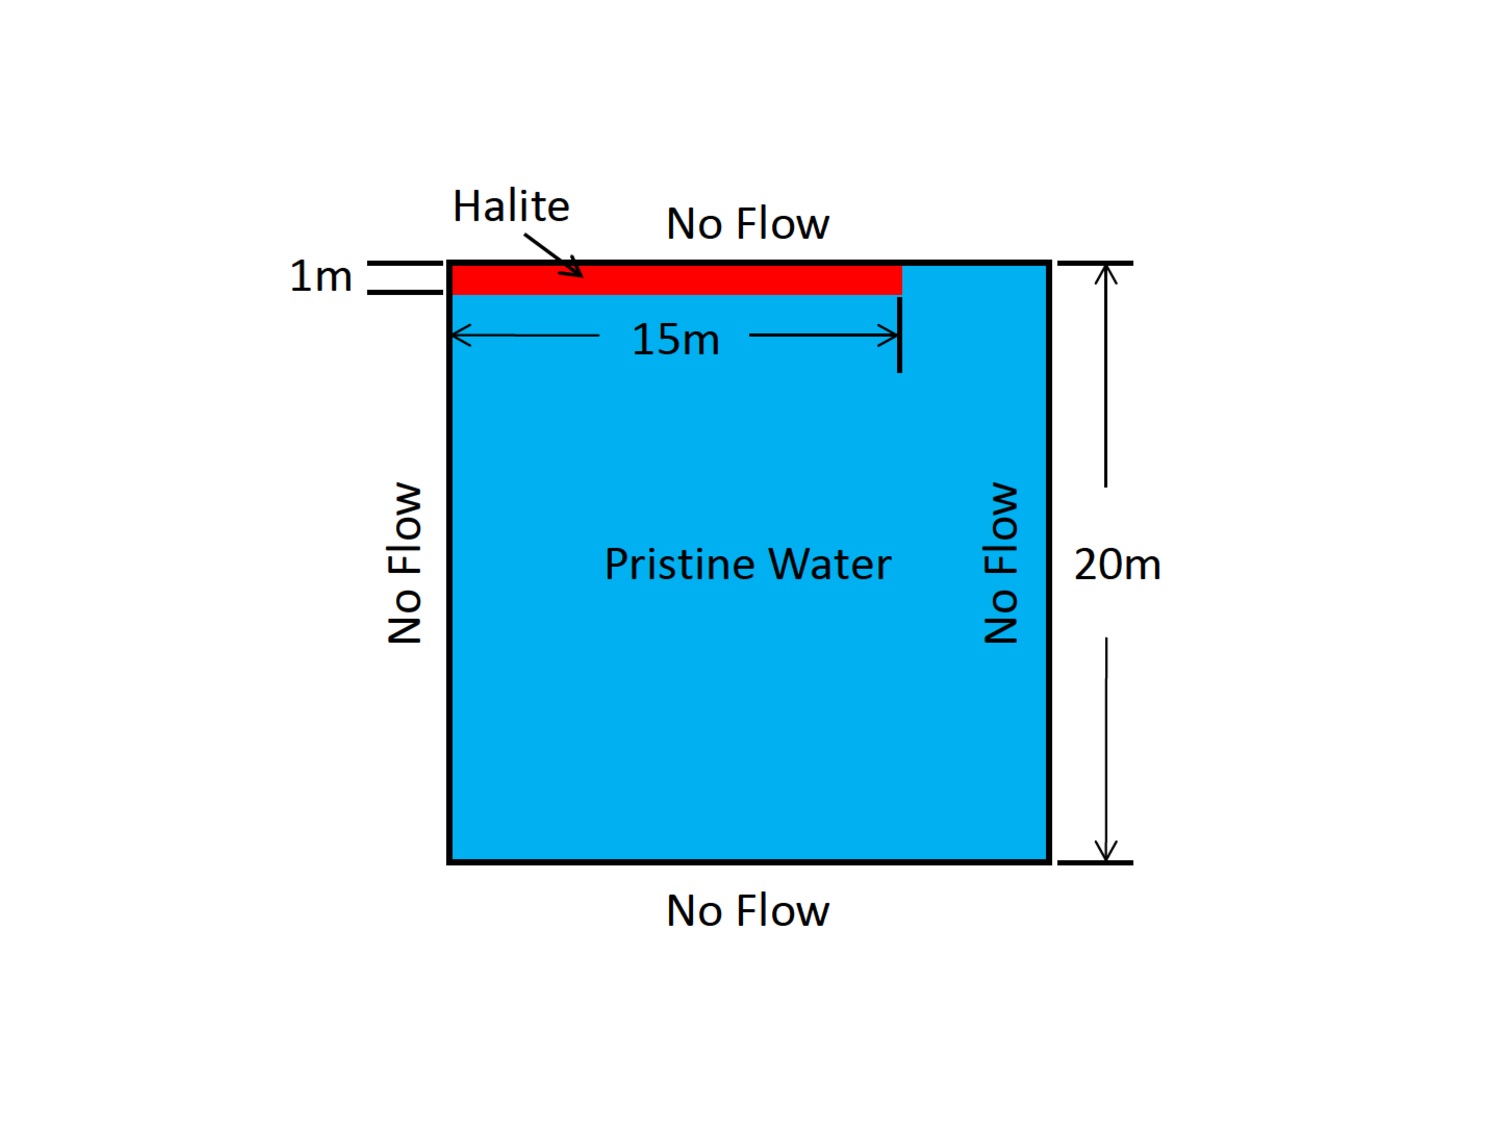
\includegraphics[width=0.75\linewidth]{./density_dependent_flow_fig}
}

%-----------------------------------------------------------------------------
\subsection{Flow Governing Equations}

\frame{\frametitle{Governing Flow Equations}

{\bf Continuity Equation:}
\EQ
\frac{\p}{\p t} \big(\varphi \rho\big) + \bnabla\cdot\rho\bq \eq 0
\EN


{\bf Darcy's Law:}
\EQ
\bq \eq -\frac{\bk}{\mu} \bnabla\big(\pressure-\rho g z\big)
\EN

\normalsize

\begin{columns}[c]
\column{0.5\linewidth}
\begin{itemize}
\item $\varphi \eq $ porosity
\item $\rho \eq $ liquid density
\item $\bk \eq $ intrinsic permeability
\item $\mu \eq $ viscosity
\end{itemize}
\column{0.5\linewidth}
\begin{itemize}
\item $\pressure \eq $ liquid pressure
\item $g \eq $ gravity
\item $z \eq $ distance in direction of gravity
\end{itemize}
\end{columns}

}

%-----------------------------------------------------------------------------
\frame{\frametitle{Constitutive Relations
%\dblline
}
\scriptsize
Batzle, M and Z. Wang, (1992) Seismic properties of pore fluids, Geophysics, V57, N11, P 1396-1408.
\small

\vspace{0.2cm}
Water Density
\vspace{-0.2cm}
\BA
\rho_w \eq 1 + 1 \times 10^{-6} \big(&-80T - 3.3T^2 + 0.00175T^3 + 489P \\
   &-2TP + 0.016T^2P - 1.3 \times 10^{-5}T^3P \\
   &-0.333 P^2 - 0.002TP^2 \big)
\EA
Brine Density
\vspace{-0.2cm}
\BA
\rho_b \eq \rho_w + S \big(& 0.668 + 0.44S + 1 \times 10^{-6} \big( 300P - \\
  &2400 PS + T \big( 80 + 3T -3300S -13P + 47PS \big)\big)\big)
\EA
Brine Viscosity
\vspace{-0.2cm}
\BA
\eta_b \eq 0.1 + &0.333S + \big(1.65 + 91.9 S^3\big) \\
&\exp\big(-\big(0.42\big(S^{0.8} - 0.17\big)^2 + 0.045\big) T^{0.8} \big)
\EA

$P$ = pressure [Pa], $T$ = temperature [C], $S$ = salt mass fraction [-]
}

%-----------------------------------------------------------------------------
\subsection{Transport Governing Equations}

\frame{\frametitle{Governing Transport Equations}


\begin{itemize}
  \item Solute transport
  \item Mineral precipitation-dissolution
\end{itemize}
  
\EQ
\frac{\p}{\p t}\big(\phi \Psi_j\big) +
\nabla\cdot\big(\qbs - \phi \Dbs\bnabla\big)\Psi_j
\eq \nu_{jm} A_m k_m  \Big(1-\frac{Q_m}{K_m}\Big)
\EN
  
\begin{columns}[c]
  \column{0.5\linewidth}
  \begin{itemize}
    \item $\varphi \eq $ porosity
    \item $\Psi_j \eq $ concentration of species $j$
    \item $\qbs \eq $ Darcy velocity
    \item $\Dbs \eq $ hydrodynamic dispersion coefficient
    \item $\nu_{jm} \eq $ stoichiometry
  \end{itemize}
  \column{0.5\linewidth}
  \begin{itemize}
    \item $A_m \eq $ specific surface area for mineral $m$
    \item $k_m \eq $ kinetic rate constant
    \item $Q_m \eq $ ion activity product
    \item $K_m \eq $ equilibrium constant
  \end{itemize}
\end{columns}  
}

%-----------------------------------------------------------------------------
\frame{\frametitle{Flow and Transport Boundary Conditions}

\begin{itemize}
\item No Flow
\item Zero Flux
\end{itemize}


}

%-----------------------------------------------------------------------------
\section{Description of Input Deck}

\subsection{SIMULATION}
\begin{frame}[fragile,containsverbatim]\frametitle{SIMULATION}

\begin{semiverbatim}
SIMULATION
  SIMULATION_TYPE SUBSURFACE
  PROCESS_MODELS
    SUBSURFACE_FLOW flow
      MODE RICHARDS
    /
    SUBSURFACE_TRANSPORT transport
      GLOBAL_IMPLICIT
    /
    \magentacomment{AUXILIARY SALINITY
      SPECIES Na+ 22.9898    \bluecomment{! formula weight of species}
      SPECIES Cl- 35.4527
    /}
  /
END
\end{semiverbatim}

\end{frame}

%-----------------------------------------------------------------------------
\subsection{CHEMISTRY}

\begin{frame}[fragile,allowframebreaks]\frametitle{CHEMISTRY}
\begin{semiverbatim}
CHEMISTRY
  PRIMARY_SPECIES
    Na+
    Cl-
  /
  MINERALS
    Halite
  /
  MINERAL_KINETICS
    Halite
      \bluecomment{# Alkattan, Oelkers et al. (1997) Experimental
      #  Studies of Halite Dissolution Kinetics}
      RATE_CONSTANT 1.d-7 mol/cm^2-sec 
    /
  /
  
  LOG_FORMULATION
  DATABASE ./density_dep_flow_database.dat
  OUTPUT
    ALL
    TOTAL
  /
END
\end{semiverbatim}

\end{frame}

%-----------------------------------------------------------------------------
\subsection{FLUID\_PROPERTY}

\begin{frame}[fragile,containsverbatim]\frametitle{FLUID\_PROPERTY}

\begin{itemize}
  \item Assign a molecular diffusion coefficient of $10^{-10}$ m$^2$/s to all aqueous species
\end{itemize}

\begin{semiverbatim}
  
FLUID_PROPERTY
  DIFFUSION_COEFFICIENT 1.d-10   \bluecomment{! [m^2/s]}
END
\end{semiverbatim}

\end{frame}

%-----------------------------------------------------------------------------
\subsection{EOS}

\begin{frame}[fragile,containsverbatim]\frametitle{EOS}

\begin{itemize}
\item Employ Batzle and Wang equation of state for water/brine
\end{itemize}

\begin{semiverbatim}

EOS WATER
  DENSITY BATZLE_AND_WANG
  VISCOSITY BATZLE_AND_WANG
END
\end{semiverbatim}

\end{frame}

%-----------------------------------------------------------------------------
\begin{frame}[fragile,containsverbatim]\frametitle{GRID}

\begin{itemize}
  \item Problem domain: $20 \times 1 \times 20$ m (x $\times$ y $\times$ z)
  \item Grid resolution $0.2 \times 1 \times 0.2$ m
\end{itemize}

\begin{semiverbatim}
GRID
  TYPE structured 
  NXYZ 100 1 100
  BOUNDS
    0.d0 0.d0 0.d0
    20.d0 1.d0 20.d0 
  /
END
\end{semiverbatim}

\end{frame}

%-----------------------------------------------------------------------------
\subsection{REGION}

\begin{frame}[fragile,containsverbatim]\frametitle{REGION}

\begin{itemize}
  \item Delineate regions in the 2D domain for:
  \begin{itemize}
    \item all (entire domain)
    \item halite\_long\_top
  \end{itemize}
  \item Although 2D, regions must still be in 3D.
\end{itemize}

\begin{semiverbatim}
REGION all
  COORDINATES
    \magentacomment{-1.d20 -1.d20 -1.d20}   
    \magentacomment{1.d20 1.d20 1.d20}      
  /
END

REGION halite\_along\_top
  COORDINATES
    0.d0 \magentacomment{-1.d20} 19.d0
    15.d0 \magentacomment{1.d20} 20.d0
  /
END
\end{semiverbatim}

\end{frame}


%-----------------------------------------------------------------------------
\subsection{MATERIAL\_PROPERTY}

\begin{frame}[fragile,containsverbatim]\frametitle{MATERIAL\_PROPERTY}

\small
\begin{semiverbatim}
MATERIAL_PROPERTY aquifer
  ID 1
  CHARACTERISTIC_CURVES sf1
  POROSITY  0.25d0
  TORTUOSITY 0.1d0
  PERMEABILITY
    PERM_ISO 1.d-12
  /
END
  
MATERIAL_PROPERTY halite
  ID 2
  CHARACTERISTIC_CURVES sf1
  POROSITY  0.15d0
  TORTUOSITY 0.1d0
  PERMEABILITY
    PERM_ISO 1.d-16
  /
END
\end{semiverbatim}

\end{frame}

%-----------------------------------------------------------------------------
\subsection{CHARACTERISTIC\_CURVES}

\begin{frame}[fragile]\frametitle{CHARACTERISTIC\_CURVES}
\begin{itemize}
\item Characteristic curve ``DEFAULT'' enables one to skip the definition of saturation and relative permeability functions for saturated flow.
\end{itemize}
\begin{semiverbatim}


CHARACTERISTIC_CURVES sf1
  DEFAULT  \bluecomment{! Must ensure that domain never becomes }
END        \bluecomment{!   variably-saturated!}
\end{semiverbatim}

\end{frame}

%-----------------------------------------------------------------------------
\subsection{OUTPUT}

\begin{frame}[fragile]\frametitle{OUTPUT}

\begin{semiverbatim}
  
OUTPUT
  NO_PRINT_INITIAL         \bluecomment{! Skip output at time 0}
  SNAPSHOT_FILE
    FORMAT HDF5 
    TIMES y 1.d-2          \bluecomment{! First output at 0.01 years}
    PERIODIC TIME 1.d0 y
    VARIABLES
      LIQUID_PRESSURE
      LIQUID_DENSITY
    /
  /
END
  
\end{semiverbatim}

\end{frame}

%-----------------------------------------------------------------------------
\subsection{TIME}

\begin{frame}[fragile]\frametitle{TIME}

\begin{itemize}
  \item Set final simulation time to 100 years
  \item Set initial time step size to 1.e-4 days
  \item Set maximum time step size to 100 days
\end{itemize}


\begin{semiverbatim}
TIME
  FINAL_TIME 100.d0 y
  INITIAL_TIMESTEP_SIZE 1.d-4 d
  MAXIMUM_TIMESTEP_SIZE 100.d0 d
END
\end{semiverbatim}

\end{frame}

%-----------------------------------------------------------------------------
\subsection{FLOW\_CONDITION}

\begin{frame}[fragile]\frametitle{FLOW\_CONDITION}

\centering
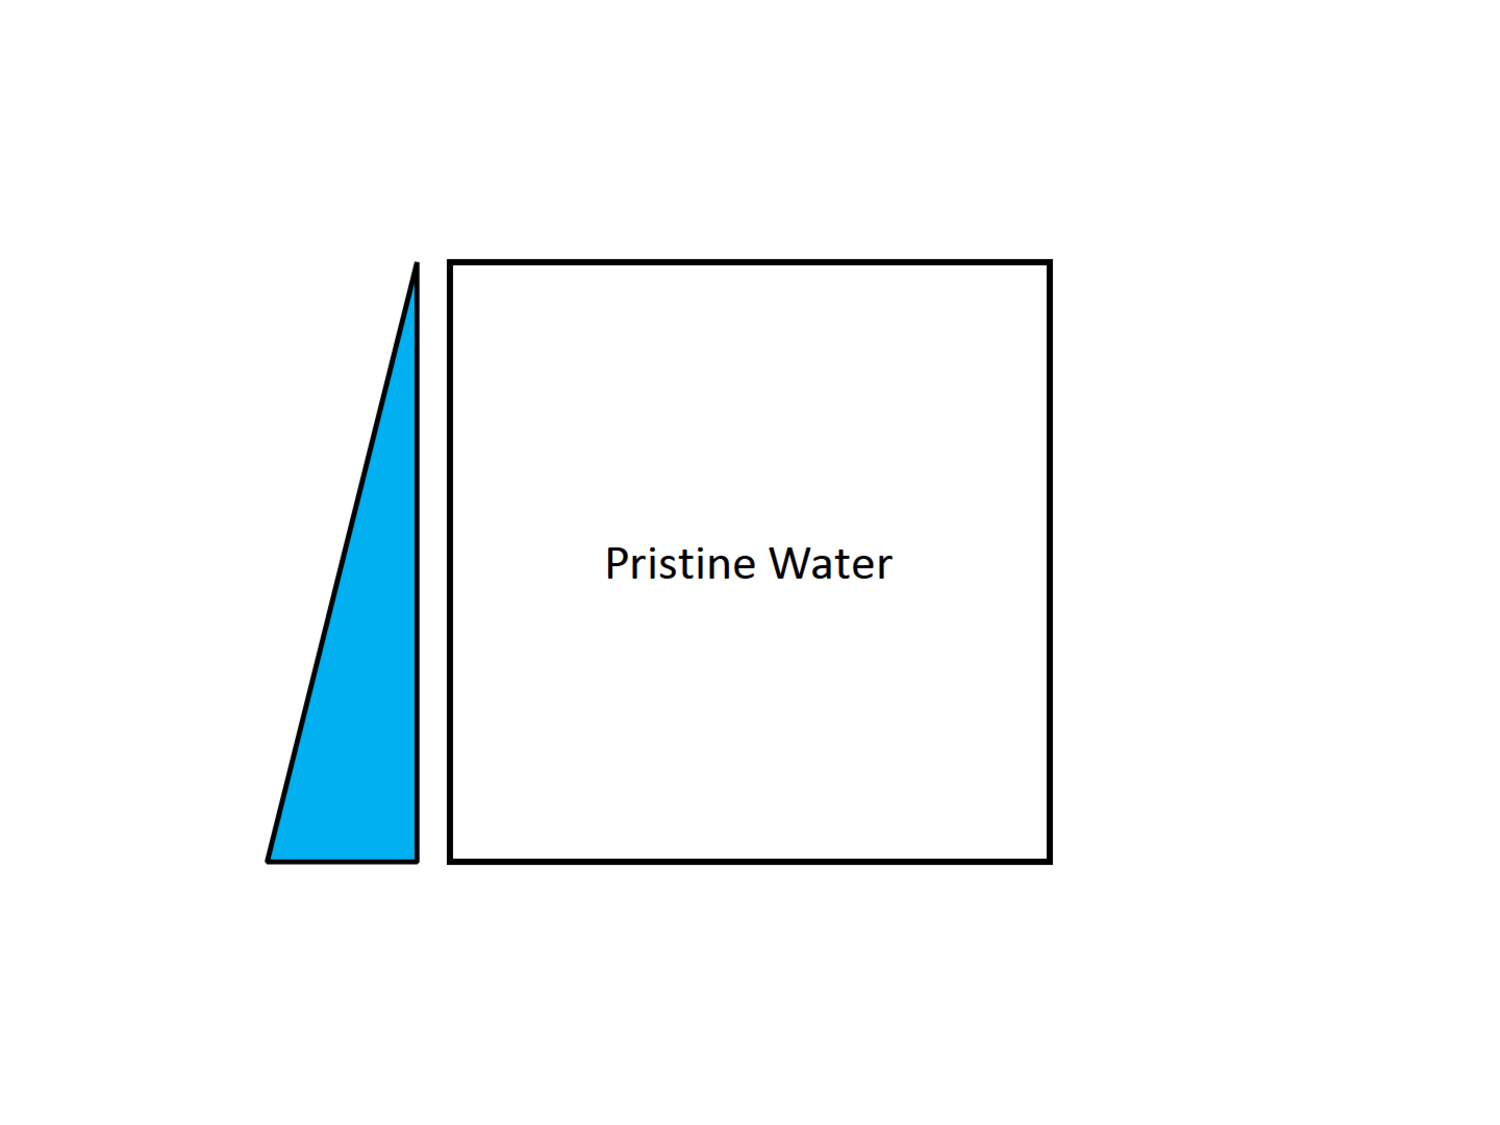
\includegraphics[width=0.35\linewidth]{./density_dependent_hydrostatic_fig}

\begin{semiverbatim}
FLOW_CONDITION initial
  TYPE
    PRESSURE HYDROSTATIC  \bluecomment{! hydrostatic condition}
  /
  DATUM 0.d0 0.d0 20.d0   \bluecomment{! point in space}
  PRESSURE 150000.d0      \bluecomment{! pressure at datum}
END
\end{semiverbatim}
\end{frame}

%-----------------------------------------------------------------------------
\subsection{TRANSPORT\_CONDITION / CONSTRAINT}

\begin{frame}[fragile,allowframebreaks]\frametitle{TRANSPORT\_CONDITION / CONSTRAINT}

{
\begin{semiverbatim}

TRANSPORT_CONDITION halite_initial
  TYPE dirichlet_zero_gradient
  CONSTRAINT halite_constraint
    CONCENTRATIONS
      Na+ 7.533d0  T
      Cl- 7.533d0  T
    /
    MINERALS
      Halite 0.85 1.0    \bluecomment{! default units of specific}
    /                    \bluecomment{! surface area are in m^2/m^3}
  /
END

\newpage
TRANSPORT_CONDITION aquifer_initial
  TYPE dirichlet_zero_gradient
  CONSTRAINT aquifer_constraint
    CONCENTRATIONS
      Na+ 1.d-6  T
      Cl- 1.d-6  T    
    /
  /
END
\end{semiverbatim}
}

\end{frame}

%-----------------------------------------------------------------------------
\subsection{BOUNDARY\_CONDITION}

\begin{frame}[fragile]\frametitle{BOUNDARY\_CONDITION}

\begin{itemize}
  \item No boundary conditions as this is a closed system.
\end{itemize}

\begin{semiverbatim}
INITIAL_CONDITION aquifer_ic
  FLOW_CONDITION initial
  TRANSPORT_CONDITION aquifer_initial
  REGION all
END

INITIAL_CONDITION halite_ic
  FLOW_CONDITION initial
  TRANSPORT_CONDITION halite_initial
  REGION halite_along_top
END
\end{semiverbatim}

\end{frame}

%-----------------------------------------------------------------------------
\subsection{STRATA}

\begin{frame}[fragile]\frametitle{STRATA}

\begin{itemize}
\item Couple material types with regions
\end{itemize}

\begin{semiverbatim}
STRATA
  MATERIAL aquifer
  REGION all
END

STRATA
  MATERIAL halite
  REGION halite_along_top
END
\end{semiverbatim}

\end{frame}



%-----------------------------------------------------------------------------
\subsection{Running density_dependent_flow.in}

\begin{frame}[fragile]\frametitle{Running PFLOTRAN}

\begin{semiverbatim}

> cd $PFLOTRAN_DIR
> cd shortcourse/exercises/density_dependent_flow
> pflotran -input_prefix density_dependent_flow

\end{semiverbatim}

\end{frame}

\end{document}
